%% CSD319 project report (acmart sigconf, two column). Compile with pdfLaTeX on Overleaf.
\documentclass[sigconf,nonacm]{acmart}
\settopmatter{printacmref=false, printccs=false, printfolios=true, authorsperrow=4}
\renewcommand\footnotetextcopyrightpermission[1]{}

\usepackage{tikz}
\usepackage{array}
\usepackage{enumitem}
\usepackage{algorithm}
\usepackage{algpseudocode}
\setlist{nosep,leftmargin=1.3em}
\emergencystretch=1.5em

\newcommand{\DED}{\textsc{DED}}
\newcommand{\Unif}{\mathrm{U}}
\newcommand{\E}{\mathbb{E}}

\begin{document}

\title{Randomized Rounding for Minimum-Weight Edge Deletion in DAGs}
\subtitle{CSD319 Design and Analysis of Algorithms: Project Report}

\author{Gaurav Rai}
\affiliation{\institution{2410110133}\country{}}
\author{Shaurya Sharma}
\affiliation{\institution{2410110317}\country{}}
\author{Sharanya Gupta}
\affiliation{\institution{2410110315}\country{}}
\author{Kashvi Tak}
\affiliation{\institution{2410110165}\country{}}

\begin{abstract}
We study the DAG Edge Deletion problem. We are given a weighted DAG and a number $k$, and we want to delete the cheapest set of edges so that no path with $k$ edges is left. The best known algorithm, by Kalantarzadeh, Klein and Reis (APPROX 2025), rounds a linear program using random vertex labels and gets a ratio of $0.549(k+1)$. Under the Unique Games Conjecture nothing better than $\lfloor k/2\rfloor$ is possible. In this report we go through that algorithm and the earlier ones, and prove why they work and how fast they run. We then tried to push the method further. We found a label distribution that gives about $0.5445(k+1)$. We also show that no distribution of this kind can do better than $0.5431(k+1)$, and that the ratio $0.5(k+1)$ is possible whenever the DAG comes with a 3-colouring. Finally, we show that this approach cannot reach $0.5(k+1)$ on every DAG. Our code is at: \url{https://github.com/gauravrai1704/DAG}.
\end{abstract}

\maketitle

\section{Problem Statement}

Let $G=(V,A)$ be a directed acyclic graph, let every edge $e$ have a cost $c_e\ge0$, and fix an integer $k\ge2$. The length of a path is its number of edges. In \DED$(k)$ we want a set $S\subseteq A$ of minimum total cost such that $G-S$ has no path of length $k$.

A simple example explains where this comes up. Think of vertices as tasks and an edge $u\to v$ as ``$u$ should finish before $v$''. If we have $k$ time steps and as many machines as we like, we can finish everything only if the longest chain of constraints has fewer than $k$ edges. When it doesn't, we have to break some constraints, and \DED$(k)$ asks for the cheapest ones to break.

There is a second way to look at the problem that we use throughout. A DAG has no path of length $k$ exactly when we can give each vertex a level $\ell(v)\in\{1,\dots,k\}$ so that every edge goes from a lower level to a higher one (put $v$ at level $1+{}$the longest path ending at $v$). So the problem is the same as splitting the vertices into $k$ layers while paying for every edge that does not go strictly forward.

\textbf{A small example.} Take the path $a\to b\to c\to d$ with edge costs $5,1,5$, and let $k=2$. The path has 3 edges, so we must cut it into pieces of at most one edge each. Deleting only the middle edge leaves $a\to b$ and $c\to d$, which costs 1. That is optimal. In terms of levels, it means putting $a,c$ on level 1 and $b,d$ on level 2. Only $b\to c$ goes backwards, so only it is paid for.

The graph has to be acyclic. On a general digraph with $k=n-1$, even deciding whether any edge needs to be deleted is the Hamiltonian Path problem. On a DAG, the longest path can be found by dynamic programming. We also allow $k$ to depend on $n$, so we want running time polynomial in both.

\textbf{The linear program.} Every algorithm in this report starts from the LP of Kenkre et al.~\cite{kpps}. There is a variable $x_e$ for each edge, which we can think of as ``how much $e$ is deleted'':
\begin{align*}
\min\ &\textstyle\sum_e c_ex_e\\
\text{s.t.}\ &\textstyle\sum_{e\in P}x_e\ge1\quad\text{for every path $P$ of length $k$},\\
&x_e\ge0\quad\text{for every edge $e$}.
\end{align*}
Any valid deletion set gives a feasible 0/1 solution, so the LP value is at most OPT. Table~\ref{tab:known} lists what was known before we started.

\begin{table}[t]
\caption{Known results for \DED$(k)$.}\label{tab:known}
\small
\begin{tabular}{@{}>{\raggedright\arraybackslash}p{0.40\columnwidth}>{\raggedright\arraybackslash}p{0.55\columnwidth}@{}}
\toprule
Bound & Source and idea\\
\midrule
$k$ & Kenkre et al.~\cite{kpps}: delete edges with $x_e\ge1/k$\\
$\tfrac23(k+1)$ & Klein and Wexler~\cite{kw}: threshold plus random 3 levels\\
$0.586(k+1)$ & KKR~\cite{kkr}: uniform random labels\\
$0.549(k+1)$ & KKR~\cite{kkr}: tuned random labels\\
$0.5(k+1)$, bipartite DAGs & KKR~\cite{kkr}: correlated labels\\
\midrule
no $\lfloor k/2\rfloor-\varepsilon$ (UGC) & \cite{kpps}, building on Svensson~\cite{sv}\\
no $\sqrt2-\varepsilon$ (NP), $k\ge4$ & reduction from Vertex Cover\\
LP gap at least $(k+1)/2$ & Klein and Wexler~\cite{kw,abglsc}\\
\bottomrule
\end{tabular}
\end{table}

\section{Algorithms}

\subsection{A first try: threshold rounding}
Solve the LP and delete every edge with $x_e\ge1/k$. Each path of length $k$ has $k$ edges whose values add up to at least 1, so one of them is at least $1/k$, and the path is broken. An edge we delete had $x_e\ge 1/k$, so its cost is at most $k\cdot c_ex_e$. This gives a factor of $k$. It is the best this rule can do: on a single path with every $x_e=1/k$, it deletes all $k$ edges when one would have been enough. The rule looks at each path separately, and that is the reason it loses so much.

\subsection{Klein and Wexler: threshold, then random levels}
Klein and Wexler~\cite{kw} were the first to beat $k$. They first delete every edge with $x_e\ge\tau$, where $\tau=\frac{3}{2(k+1)}$. Then they put every vertex on a random level from $\{1,2,3\}$ and delete the remaining edges with $x_e>0$ that do not go forward. The idea of using random levels is what KKR later made continuous.

\subsection{Rounding with random labels}
The algorithm of Kalantarzadeh, Klein and Reis~\cite{kkr} (KKR from now on) fixes this by making one global random choice. Each vertex gets a real label in $[0,1]$, which we can think of as a ``soft level''. An edge is deleted when it does not climb enough, where the amount it needs to climb depends on its LP value (Algorithm~\ref{alg:kkr}).

\begin{algorithm}[t]
\caption{Label rounding for \DED$(k)$}\label{alg:kkr}
\begin{algorithmic}[1]
\Require DAG $G=(V,A)$, costs $c$, integer $k$, label distribution $\mu$
\State solve the LP and get $x$
\State draw labels $\ell\in[0,1]^V$ from $\mu$
\State $S\gets\{(u,v)\in A:\ \ell(v)-\ell(u)\le(k+1)x_{uv}-1\}$
\State \Return $S$
\end{algorithmic}
\end{algorithm}

Edges with large $x_e$ are deleted easily, and edges with $x_e=0$ are deleted only if their label difference is exactly $-1$. If all labels are set to $0$, the rule becomes ``delete if $x_e\ge1/(k+1)$'', which is almost the threshold rule. So threshold rounding is a special case. The whole question is which distribution $\mu$ to use.

\textbf{Uniform labels.} The simplest choice is to give each vertex an independent uniform label in $[0,1]$. This gives a ratio of $(2-\sqrt2)(k+1)\approx0.586(k+1)$.

\textbf{KKR's tuned labels.} KKR use the density $p(x)=\frac23+\frac{23}3(1-2x)^{22}$, which puts more weight near $0$ and $1$. They found it by computer search, and it gives $0.549(k+1)$.

\textbf{Our step labels.} We tried to find a better density with an optimiser. We split $[0,1]$ into $N$ equal pieces and let the density be constant on each piece, with weights $p_1,\dots,p_N$. For this kind of density the difference $X-Y$ of two labels has an exact formula,
\[
\Pr[X-Y\le t]=\textstyle\sum_d c_d\,T(Nt-d),\qquad c_d=\sum_{i-j=d}p_ip_j,
\]
where $T$ is the CDF of the triangle distribution on $[-1,1]$. This made the search fast. We ran L-BFGS from several starting points, one of them KKR's density. With $N=24$ we got a ratio of $0.54499(k+1)$, and with $N=48$ we got $0.5446(k+1)$. The best density still has a lot of weight at the two ends (about $7\%$ in the first piece and $24\%$ in the last), but unlike KKR's it is not symmetric.

\textbf{Correlated labels.} The labels do not have to be independent. For a bipartite DAG, KKR pick $y$ uniformly from $[0,1]$, give one side label $0$ and the other side label $y$, and flip a coin to decide which side is which. We noticed that the same idea works with three colours. Given a proper 3-colouring of the DAG (ignoring edge directions), pick $Y$ uniformly from $[0,1]$ and hand out the three values $0$, $Y$ and $1-Y$ to the three colour classes in a random order. Both of these give ratio $0.5(k+1)$ (Section~\ref{sec:proofs}).

\section{Proof of Correctness}\label{sec:proofs}

\subsection{Threshold and Klein--Wexler are valid}
For threshold rounding this was shown in Section~2.1. For Klein and Wexler, take a path of length $k$ that survives the first step. All its edges have $x_e<\tau$ and the values add up to at least 1. So more than $1/\tau=\frac23(k+1)$ of its edges have $x_e>0$, and fewer than $\frac{k-2}3$ have $x_e=0$. The zero edges split the path into fewer than $\frac{k+1}3$ runs of positive edges, so the average run is longer than 2 edges. Some run then has at least 3 edges, and three random levels can never keep three edges in a row going forward. So the path gets broken.

The cost analysis uses the following fact. We give a short proof of our own.
\begin{lemma}\label{lem:avg}
If $x$ is an optimal LP solution and $L=\{e:x_e>0\}$, then $\sum_{e\in L}c_e\le k\cdot\sum_ec_ex_e$.
\end{lemma}
\begin{proof}
For a small $\delta>0$ let $y_e=(1+\delta)x_e-\delta/k$ on $L$ and $y_e=0$ elsewhere. A path of length $k$ contains at most $k$ edges of $L$, so its $y$-sum is at least $(1+\delta)\cdot1-\delta=1$. So $y$ is feasible, and optimality of $x$ gives $c(y)\ge c(x)$, which simplifies to the claim.
\end{proof}

\subsection{The output of label rounding is always valid}
\begin{lemma}\label{lem:feas}
For any feasible $x$ and any labels $\ell\in[0,1]^V$, Algorithm~\ref{alg:kkr} leaves no path of length $k$.
\end{lemma}
\begin{proof}
Suppose a path $P$ of length $k$ from $a$ to $b$ survives. Every edge on it was kept, so $\ell(\text{head})-\ell(\text{tail})>(k+1)x_e-1$ for each $e\in P$. Adding these up, the left side telescopes:
\[\ell(b)-\ell(a)>(k+1)\textstyle\sum_{e\in P}x_e-k\ge(k+1)-k=1.\]
But both labels are in $[0,1]$, so their difference is at most 1. This is a contradiction.
\end{proof}

\subsection{The cost bound}
Let $Z_e=\ell(v)-\ell(u)$ for an edge $e=(u,v)$.
\begin{lemma}\label{lem:cost}
Let $\alpha\ge\frac12$. Suppose that for every edge and every $t\in[-1,1]$,
\[(C_\alpha):\qquad\Pr[Z_e\le t]\le\alpha(1+t).\]
Then the expected cost of the output is at most $\alpha(k+1)\cdot\mathrm{OPT}$.
\end{lemma}
\begin{proof}
Edge $e$ is deleted when $Z_e\le t$ with $t=(k+1)x_e-1$. If $t\le1$, condition $(C_\alpha)$ gives $\Pr[e\text{ deleted}]\le\alpha(k+1)x_e$. If $t>1$, then $x_e>2/(k+1)$, so $\alpha(k+1)x_e>2\alpha\ge1$, and the bound holds trivially. By linearity of expectation the expected cost is at most $\alpha(k+1)\sum_ec_ex_e\le\alpha(k+1)\cdot\mathrm{OPT}$.
\end{proof}

So the analysis comes down to one random variable per edge. At $t=1$ the condition forces $\alpha\ge\frac12$. If $Z_e$ is symmetric, $(C_\alpha)$ also bounds the CDF from below by $1-\alpha(1-t)$, and at $\alpha=\frac12$ the two bounds meet. In other words, $\frac12(k+1)$ needs every $Z_e$ to be \emph{exactly} uniform on $[-1,1]$. This one fact guided most of our work.

\textbf{Uniform labels give $2-\sqrt2$.} If both labels are uniform, $Z$ has the triangle distribution, with $\Pr[Z\le t]=1-(1-t)^2/2$ for $t\ge0$. Setting the derivative of $\Pr[Z\le t]/(1+t)$ to zero gives $t^2+2t-1=0$, so $t=\sqrt2-1$ and the ratio is $2-\sqrt2$. For $t<0$ the ratio is at most $\frac12$. We checked this and KKR's value of $0.5482$ numerically and got the same numbers.

\textbf{Our step density.} Since the CDF of $Z$ only goes up, on any small interval $[t_0,t_1]$ we have $\Pr[Z\le t]/(1+t)\le\Pr[Z\le t_1]/(1+t_0)$. We evaluated this bound on $4$ million intervals, with the weights stored as exact fractions, and got $0.544510$ for $N=48$. We also checked it with $2\times10^7$ random samples.

\begin{theorem}\label{thm:3col}
Given a DAG with a proper 3-colouring $\chi$ of its underlying undirected graph, the three-value labelling from Section~2.2 makes Algorithm~\ref{alg:kkr} a $\frac12(k+1)$-approximation.
\end{theorem}
\begin{proof}
An edge joins two different colours. The order in which the values are handed out is random, so the pair (tail label, head label) is equally likely to be any of the 6 ordered pairs of distinct values from $\{0,Y,1-Y\}$. The difference is then $Y$, $-Y$, $1-Y$, $Y-1$, $1-2Y$ or $2Y-1$, each with probability $\frac16$. Since $Y$ is uniform on $[0,1]$, the first four together are uniform on $[-1,1]$, and so are the last two. So $Z_e$ is exactly uniform on $[-1,1]$, $(C_{1/2})$ holds, and we use Lemmas~\ref{lem:feas} and~\ref{lem:cost}.
\end{proof}
The bipartite case of KKR is the same proof with only the values $\{0,Y\}$. Some classes where a 3-colouring is easy to find are DAGs of maximum degree 3 (except $K_4$), and outerplanar and series-parallel DAGs.

\subsection{How well can any algorithm do?}
There are two kinds: hardness results, which hold for every polynomial-time algorithm, and integrality gaps, which hold for every algorithm that compares itself to this LP.

\textbf{Hardness.} Svensson~\cite{sv} studied the vertex version of the problem, where we delete vertices instead of edges so that no path with $t$ vertices is left. Assuming the Unique Games Conjecture, he showed it is hard to tell apart two kinds of DAGs. In the first kind, removing about $|V|/t$ vertices is enough. In the second kind, almost all vertices must be removed. So no algorithm can approximate the vertex version within $t-\varepsilon$.

Kenkre et al.~\cite{kpps} turn this into a result for edges with a simple gadget. Set $t=\lfloor k/2\rfloor$. Split every vertex $v$ into two vertices $v_{\text{in}}\to v_{\text{out}}$ joined by an edge of cost 1. Every original edge $u\to v$ becomes $u_{\text{out}}\to v_{\text{in}}$ and gets a very large cost, so no good solution deletes it. Deleting the edge $v_{\text{in}}\to v_{\text{out}}$ now plays the role of deleting the vertex $v$.
\begin{itemize}
\item A path in the new graph alternates between split edges and original edges. So a path of $2t\le k$ edges passes through $t$ split edges, that is, through $t$ old vertices. If the deleted vertices broke every $t$-vertex path in the old graph, then every $k$-edge path in the new graph is broken too, at the same cost.
\item In the other direction, a path through $t+1$ old vertices becomes a path of $2t+1\ge k$ edges. So any valid edge deletion also gives a valid vertex deletion of the same cost.
\end{itemize}
The costs are the same in both directions, so the gap of about $t$ carries over. Hence \DED$(k)$ cannot be approximated better than $\lfloor k/2\rfloor-\varepsilon$ for constant $k\ge4$, assuming the UGC. The gadget graph is bipartite (in-copies on one side, out-copies on the other), which is why the $\frac12(k+1)$ bipartite algorithm is essentially the best possible on these instances.

\textbf{Integrality gap.} The ratio of every LP-based algorithm in this report is measured against the LP value. So none of them can beat the worst ratio $\mathrm{OPT}/\mathrm{LP}$ over all instances. Klein and Wexler~\cite{kw} showed that this ratio can be close to $\frac{k+1}2$, using a graph of Alon et al.~\cite{abglsc}:
\begin{itemize}
\item Choose a set $A$ of $r\approx n^{1/3}$ integers whose pairwise differences are all different. On the vertices $0,1,\dots,n-1$ (arithmetic mod $n$), add an edge $i+a\to i+b$ for every $i$ and every $a<b$ in $A$.
\item The edges form $n$ cliques of size $r$ that share no edges. When the vertices are split into $k$ levels, at most a $\frac{k-1}{k}$ fraction of the edges inside each clique join two different levels.
\item Every vertex has the same in-degree and out-degree. Because of this, at most half of those edges go forward. So any solution keeps at most about $\frac{k-1}{2k}$ of the edges, and must delete at least about $\frac{k+1}{2k}$ of them.
\item The graph is not quite acyclic, because of the edges that wrap around modulo $n$. There are only $O(r^4)$ of them, a vanishing fraction, and deleting them makes it a DAG.
\end{itemize}
On the other hand, setting $x_e=\frac1k$ for every edge satisfies every path constraint, so the LP value is at most $\frac1k|E|$. Dividing gives $\mathrm{OPT}/\mathrm{LP}\ge\frac{k+1}{2}-o(1)$. So no rounding of this LP can guarantee better than $\frac12(k+1)$, and the gap between the best algorithm and this limit is only in the constant (0.549 or, with our labels, 0.5445, against 0.5).

\subsection{Limits of the method}

\begin{figure*}[t]
\centering
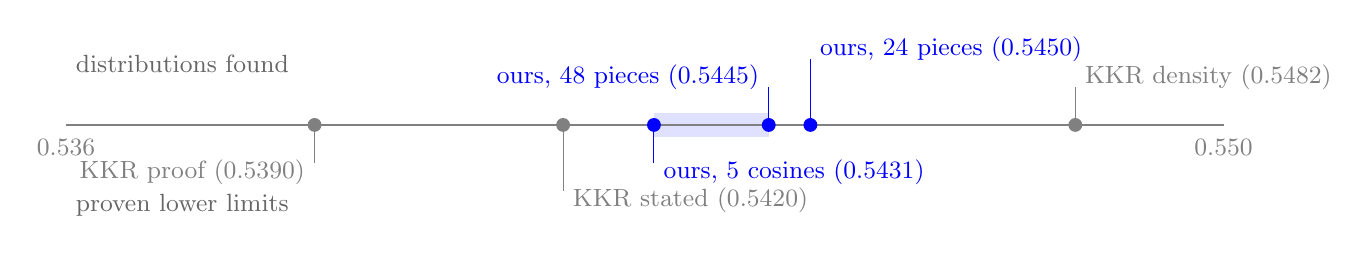
\begin{tikzpicture}[x=1.05cm,y=0.6cm,font=\small]
\fill[blue!12] ({(0.5431-0.536)*1000},-0.25) rectangle ({(0.5445-0.536)*1000},0.25);
\draw[thick,gray] (0,0) -- (14,0);
\node[below,gray] at (0,-0.1) {0.536}; \node[below,gray] at (14,-0.1) {0.550};
\foreach \v/\c/\h in {0.5390/gray/-1, 0.5420/gray/-1.6, 0.5431/blue/-1}{
  \draw[\c] ({(\v-0.536)*1000},0) -- ({(\v-0.536)*1000},\h+0.2);
  \fill[\c] ({(\v-0.536)*1000},0) circle (2.5pt);}
\foreach \v/\c/\h in {0.5445/blue/1.0, 0.5450/blue/1.6, 0.5482/gray/1.0}{
  \draw[\c] ({(\v-0.536)*1000},0) -- ({(\v-0.536)*1000},\h-0.2);
  \fill[\c] ({(\v-0.536)*1000},0) circle (2.5pt);}
\node[anchor=east,gray] at ({(0.5390-0.536)*1000},-1) {KKR proof (0.5390)};
\node[anchor=west,gray] at ({(0.5420-0.536)*1000},-1.6) {KKR stated (0.5420)};
\node[anchor=west,blue] at ({(0.5431-0.536)*1000},-1) {ours, 5 cosines (0.5431)};
\node[anchor=east,blue] at ({(0.5445-0.536)*1000},1.0) {ours, 48 pieces (0.5445)};
\node[anchor=west,blue] at ({(0.5450-0.536)*1000},1.6) {ours, 24 pieces (0.5450)};
\node[anchor=west,gray] at ({(0.5482-0.536)*1000},1.0) {KKR density (0.5482)};
\node[anchor=west,gray!80!black] at (0,1.3) {distributions found};
\node[anchor=west,gray!80!black] at (0,-1.7) {proven lower limits};
\end{tikzpicture}
\caption{Where the best constant $\alpha^*$ for independent labels can lie (the ratio is $\alpha^*(k+1)$). After KKR it was somewhere in $[0.542,0.549]$. It is now in the shaded range $[0.5431,0.5445]$.}
\label{fig:window}
\end{figure*}

\textbf{Independent labels cannot reach $\frac12$.} If $X$ and $Y$ are independent with the same distribution, then $\E\cos(t(X-Y))=|\E e^{itX}|^2\ge0$. For the uniform distribution on $[-1,1]$, however, $\E\cos(tU)=\sin t/t$, which is negative for $t\in(\pi,2\pi)$. So $X-Y$ can never be exactly uniform. KKR turn this into a number. Let $G(x)=\Pr[Z\le x]-\frac{1+x}2$. Integration by parts gives
\[\textstyle\E\cos(tZ)=\frac{\sin t}t+2t\int_0^1\sin(tx)G(x)\,dx.\]
Using $(C_\alpha)$ to bound $G$ from both sides gives $\alpha\ge\frac12+\frac{-\sin t}{6t+2\sin t}$, which is about $0.539$ at $t\approx4.49$.

We improved this by using several cosines at once. For weights $a_j\ge0$, the sum $\sum_ja_j\E\cos(t_jZ)$ is still non-negative. Repeating the same steps with $h(x)=\sum_ja_jt_j\sin(t_jx)$ gives
\[\alpha\ge\frac12+\frac{-\sum_ja_j\sin(t_j)/t_j}{2\int_0^1\big(h^+(x)(1+x)+h^-(x)(1-x)\big)dx}.\]
We optimised the weights and frequencies numerically and checked each result with careful numerical integration. Two cosines give $0.5422$ and five give $0.5431$, which is the best we found. The gain from each extra cosine was getting small, so we stopped there. One small thing we noticed: the two-cosine parameters printed in~\cite{kkr} give only $0.5388$ with this formula, although other parameters do reach their claimed $0.542$. Figure~\ref{fig:window} puts all the bounds together.

\textbf{Where colourings stop working.} Theorem~\ref{thm:3col} needs every pair of colours to have a uniform difference. With $c$ colours, $|\sum_{\text{colours}}e^{it\ell}|^2\ge0$ gives $\sin t/t\ge-1/(c-1)$. The smallest value of $\sin t/t$ is $-0.2172$, so this is only possible for $c\le5$. For 4 and 5 colours we solved LPs over label distributions restricted to the values $\{0,\frac1m,\dots,1\}$, and checked the answers with exact fractions. We got $0.5063$ for 4 colours ($m=40$) and $0.5106$ for 5 colours ($m=24$). In each case this is the same as the best possible for a single edge on that grid, which makes us think 4 and 5 colours can also reach exactly $\frac12$. We could not prove it. Since planar graphs can be 4-coloured in polynomial time, this already gives $0.5064(k+1)$ for planar DAGs.

\textbf{Correlated labels cannot fix everything.} Every DAG sits inside a complete DAG $T_n$ (edges $i\to j$ for all $i<j$). Our LPs found labels with $\alpha=\frac12$ on $T_n$ for $n\le6$, so we checked whether this keeps going.

\begin{theorem}
For $n\ge418$, no distribution of labels, independent or not, satisfies $(C_{1/2})$ on $T_n$.
\end{theorem}
\begin{proof}
Let $m_i=\E\ell(i)$. Condition $(C_{1/2})$ says the CDF of $Z_{ij}=\ell(j)-\ell(i)$ is below the uniform one, so $\E Z_{ij}\ge0$ and $m_1\le\dots\le m_n$, all in $[0,1]$. Integration by parts shows $|\E\cos(tZ_{ij})-\frac{\sin t}t|\le t(m_j-m_i)$. Now cut the vertices into $r=\lfloor n/w\rfloor$ blocks of $w$ consecutive vertices. The total increase of $m$ is at most 1, so inside some block $m_j-m_i\le 1/r$. In that block $|\sum e^{it\ell(v)}|^2\ge0$ forces the average of $\E\cos(tZ_{ij})$ over pairs to be at least $-\frac1{w-1}$. Putting these together gives $-\frac1{w-1}\le\frac{\sin t}t+\frac tr$. At $t=4.49$ and the best $w$, this fails once $n\ge418$.
\end{proof}
So this whole family of algorithms, which uses one fixed label distribution and checks each edge separately, cannot prove $\frac12(k+1)$ for all DAGs.

\section{Complexity Analysis}
\textbf{Solving the LP.} The LP has one constraint per path of length $k$, which can be exponentially many. But given $x$, we can find a violated path quickly. Let $a(v,t)$ be the smallest total $x$ over paths of $t$ edges ending at $v$. Going through the vertices in topological order,
\[a(v,t)=\min_{(u,v)\in A}\big(a(u,t-1)+x_{uv}\big),\qquad a(v,0)=0.\]
A constraint is violated exactly when some $a(v,k)<1$. This takes $O(k(|V|+|A|))$ time, so the ellipsoid method solves the LP in polynomial time. In practice we can avoid the ellipsoid method. Adding variables $d(v,t)$ with $d(v,t)\le d(u,t-1)+x_{uv}$, $d(v,0)=0$ and $d(v,k)\ge1$ gives an equivalent LP with $O(k|V|+|A|)$ variables and $O(k|A|)$ constraints, which an interior point method solves in polynomial time.

\textbf{Rounding.} Drawing the labels takes $O(|V|)$ time for every distribution in this report: one sample per vertex for independent labels, or one value of $Y$ plus a random order of the colours. Checking every edge takes $O(|A|)$. So the LP dominates the total time, which is polynomial in $n$ and $k$ with no exponential dependence on $k$. The algorithm can be made deterministic with the method of conditional expectations, losing an arbitrarily small amount.

\section{Conclusion}
\begin{table}[h]
\caption{Summary of our results.}\label{tab:ours}
\small
\begin{tabular}{@{}>{\raggedright\arraybackslash}p{0.50\columnwidth}>{\raggedright\arraybackslash}p{0.45\columnwidth}@{}}
\toprule
Result & How it was shown\\
\midrule
ratio $0.5446(k+1)$ with independent labels & search plus numerical check\\
no independent labels beat $0.5431(k+1)$ & proof plus numerical integration\\
$0.5(k+1)$ for 3-colourable DAGs & proof\\
$0.5064(k+1)$ for planar DAGs & LP checked with exact fractions\\
no single distribution reaches $0.5$ on all DAGs & proof\\
\bottomrule
\end{tabular}
\end{table}

We went through the main algorithms for \DED$(k)$ and proved their correctness and running time. The key point we took away is that KKR's analysis reduces everything to a single question: how close can the difference of two random labels get to the uniform distribution on $[-1,1]$? For independent labels, the best constant is now pinned down to $[0.5431,0.5445]$. For correlated labels, the optimal $\frac12(k+1)$ extends from bipartite DAGs to 3-colourable ones, but it cannot be reached on all DAGs with one fixed distribution.

\section{Gaps and Future Directions}
\begin{itemize}
\item \emph{A gap in an earlier proof.} When we worked through Klein and Wexler's $\frac23(k+1)$ algorithm~\cite{kw}, we could not complete the final cost step. It needs the deleted low-value edges to be paid for by their own LP value, and the lemma they use only bounds this against the whole LP. A direct calculation only gives about $0.89k$. This does not affect the newer results, which avoid that step.
\item \emph{Our numbers are not formal proofs.} The upper bound and the 4- and 5-colour results are checked carefully, but in floating point. Interval arithmetic would make them fully rigorous.
\item \emph{Closing the window.} The cosine method does not use the fact that a density is non-negative. This is probably why it levels off, as in related autoconvolution problems~\cite{cs}.
\item \emph{4 and 5 colours.} We expect explicit constructions like $\{0,Y,1-Y\}$ to exist, but we have not found them.
\item \emph{Labels that depend on $x$.} Our last theorem says a $\frac12(k+1)$ algorithm must either choose labels using the LP solution, or analyse whole paths instead of single edges.
\item \emph{Hardness.} It is still open whether any constant factor is NP-hard. A result like that would also say something new about project scheduling~\cite{sv}.
\end{itemize}

\begin{thebibliography}{9}
\bibitem{kkr} S.~Kalantarzadeh, N.~Klein, V.~Reis. A randomized rounding approach for DAG edge deletion. APPROX 2025; arXiv:2507.07943.
\bibitem{kpps} S.~Kenkre, V.~Pandit, M.~Purohit, R.~Saket. On the approximability of digraph ordering. ESA 2015; Algorithmica 78(4), 2017.
\bibitem{kw} N.~Klein (advisor T.~Wexler). On the approximability of DAG edge deletion. Thesis, 2015--16.
\bibitem{sv} O.~Svensson. Hardness of vertex deletion and project scheduling. APPROX 2012.
\bibitem{abglsc} N.~Alon, B.~Bollob\'as, A.~Gy\'arf\'as, J.~Lehel, A.~Scott. Maximum directed cuts in acyclic digraphs. J.\ Graph Theory 55(1), 2007.
\bibitem{cs} A.~Cloninger, S.~Steinerberger. On suprema of autoconvolutions with an application to Sidon sets. Proc.\ AMS 145(8), 2017.
\end{thebibliography}

\end{document}
